\documentclass[letterpaper,11pt]{article}

% Soporte para los acentos.
\usepackage[utf8]{inputenc}
\usepackage[T1]{fontenc}    
% Idioma español.
\usepackage[spanish,mexico, es-tabla]{babel}
% Soporte de símbolos adicionales (matemáticas)
\usepackage{multirow}
\usepackage{amsmath}		
\usepackage{amssymb}		
\usepackage{amsthm}
\usepackage{amsfonts}
\usepackage{latexsym}
\usepackage{enumerate}
\usepackage{ragged2e}
\usepackage{graphicx}
% Modificamos los márgenes del documento.
\usepackage[lmargin=2cm,rmargin=2cm,top=2cm,bottom=2cm]{geometry}

\title{Facultad de Ciencias, UNAM \\ 
       Reconocimiento de patrones y aprendizaje automatizado \\ 
       Tarea 1}
\author{Rubí Rojas Tania Michelle}
\date{\today}

\begin{document}
\maketitle

\begin{enumerate}
    % Ejercicio 1.
    \item Considera la siguiente expresión para calcular los elementos de un 
    conjunto de punto flotante 
    \begin{equation*}
        2(\beta - 1) \beta^{l-1} (L - l + 1) + 1
    \end{equation*}

    donde $\beta$ es la base, $L$ es el exponente más grande y $l$ el más 
    pequeño. Calcula todos los elementos para los siguientes valores 
    $\beta = 2$, $L = 2$ y $l = -1$, donde los números tienen $3$ cifras 
    significativas.

    Construye todos los números de este conjunto F.

    \textsc{Solución:}
    \begin{align*}
        2(\beta - 1) \beta^{l-1} (L - l + 1) + 1
        &= 2(2 - 1) 2^{-1-1} (2 - (-1) + 1) + 1 \\
        &= 2(3) 2^{-2} (3 + 1) + 1 \\ 
        &= 6 \left( \frac{1}{4} \right)\ (4) + 1 \\ 
        &= \left( \frac{6}{4} \right) 5 \\ 
        &= \left( \frac{3}{2} \right) 5 \\
        &= \frac{15}{2}
    \end{align*}
    
    % Ejercicio 2.
    \item Determina el condicionamiento de la siguiente función:
    \begin{equation*}
        f(x) = \sqrt{x - 1} - \sqrt{x}
    \end{equation*}

    % Ejercicio 3.
    \item Implementa los algoritmos de la bisección y de newton en un 
    script. Muestra su funcionamiento con la siguiente función 
    \begin{equation*}
        g(x) = x^3 - x - 1
    \end{equation*}

    % Ejercicio 4.
    \item Usa los métodos implementados en la pregunta $3$ para encontrar $x^*$
    que soluciona $g(x^*) = 0$ y $h(x^*) = 0$ en las siguientes funciones
    \begin{equation*}
        g(x) = cos(x) - x
    \end{equation*}

    en el intervalo $[\frac{1}{2}, 1]$, y 
    \begin{equation*}
        h(x) = x^2 - x - 1
    \end{equation*}

    en el intervalo $[1, 2]$. En este caso, la tolerancia debe ser mínimo de 
    $10^{-8}$.

    % Ejercicio 5.
    \item Muestra que el polinomio característico $p(\lambda)$ de una matriz 
    $A \in \mathcal{R}^{2 \times 2}$ se puede expresar como 
    \begin{equation*}
        p(\lambda) = \lambda^2 - \lambda tr(A) + det(A)
    \end{equation*}

    donde tr(A) es la traza de la matriz $A$ y det(A) es el determinante de la 
    misma. 

    \begin{proof}
        Sea $A = \begin{pmatrix} a & b \\ c & d \\ \end{pmatrix} \in 
        M_{2 \times 2}(R)$. Entonces, tenemos que
        \begin{align*}
            p(\lambda) 
            &= det(A - \lambda I_n)
            && \text{definición de $p(\lambda)$} \\
            &= det \left( \begin{pmatrix} a & b \\ c & d \end{pmatrix} - 
                          \lambda \begin{pmatrix} 1 & 0 \\ 0 & 1 \end{pmatrix}
                   \right) 
            && \text{multiplicación escalar de matrices} \\
            &= det \left(\begin{pmatrix} a & b \\ c & d \\ \end{pmatrix} - 
                         \begin{pmatrix} \lambda & 0 \\ 0 & \lambda \end{pmatrix} 
                   \right)
            && \text{sustituyendo valores} \\
            &= det \left( \begin{pmatrix} a - \lambda & b \\ c & d -\lambda 
                          \end{pmatrix} \right)
            && \text{resta de matrices} \\
            &= (a - \lambda) (d - \lambda) - bc
            && \text{definición del determinante} \\ 
            &= ad - a\lambda - d\lambda + \lambda^2 - bc
            && \text{álgebra} \\
            &= ad - (a + d)\lambda + \lambda^2 - bc
            && \text{factorizando} \\
            &= \lambda^2 - (a + d)\lambda + (ad - bc)
            && \text{reacomodando la expresión} \\
            &= \lambda^2 - tr(A)\lambda + det(A)
            && \text{definición de tr(A) y det(A)} \\
            &= \lambda^2 - \lambda tr(A) + det(A) 
            && \text{conmutatividad de la multiplicación}
        \end{align*}

        Por lo tanto, el polinomio característico de la matriz $A$ puede ser 
        expresado como 
        \begin{equation*}
            p(\lambda) = \lambda^2 - \lambda tr(A) + det(A)
        \end{equation*}
    \end{proof}

    % Ejercicio 6.
    \item Utiliza el algoritmo de KNN con el dataset \texttt{"trees.csv"}. Este 
    dataset cuenta con tres variables o atributos: el diámetro a la altura del 
    pecho, la altura y el volumen de varios árboles. Utilizándo los notebooks 
    provistos en clase, responde:
    \begin{enumerate}
        % Ejercicio 6.a
        \item Define dos variables independientes y una dependiente. Justifica 
        tu elección.

        \textsc{Solución:} Definimos a las variables \texttt{"Girth"} y 
        \texttt{"Height"} como independientes y a la variable \texttt{"Volume"}
        como dependiente. La elección la realizamos de esta forma porque es 
        más sencillo medir la altura y el diámetro a la altura del pecho, que 
        medir el volúmen de los árboles (estuve leyendo un poco al respecto, y 
        para calcular el volumen sin necesidad de talar el árbol se necesitan 
        algunas técnicas complicadas y muy tardadas). Por lo que, es útil poder 
        predecir el volumen del árbol a partir de la altura y el diámetro dados.

        % Ejercicio 6.b
        \item Normaliza las variables, ¿para qué hacemos esto?

        \textsc{Solución:} Para que funcionen mejor muchos algoritmos de 
        \textit{Machine Learning} hay que normalizar las variables de entrada 
        al algoritmo. Normalizar significa, en este caso, comprimir o extender 
        los valores de la variable para que estén en un rango definido.

        % Ejercicio 6.c
        \item Separa tu dataset en conjunto de entrenamiento y conjunto de 
        prueba. ¿Por qué hacemos esto?

        \textsc{Solución:} Una vez que seleccionamos el mejor modelo que se 
        puede crear con los datos disponibles, se tiene que comprobar su 
        capacidad prediciéndo nuevas observaciones que no se hayan empleado 
        para entrenarlo, de esta forma se verifica si el modelo se puede 
        generalizar. Una estrategia para hacer esto es dividir (de manera 
        aleatoria, o no) los datos en dos grupos, ajustar el modelo con el 
        primer grupo y estimar la precisión de las predicciones con el 
        segundo conjunto.

        El tamaño adecuado para las particiones depende de la cantidad de 
        datos disponibles y la seguridad que se necesite en la estimación 
        del error, pero en general dividir el conjunto en un $80-20$ 
        (entrenamiento - prueba) suele dar buenos resultados.

        % Ejercicio 6.d
        \item Encuentra la $k$ óptima para aplicar el algoritmo.
        
        \textsc{Solución:}

        % Ejercicio 6.e
        \item Obtén el MSE del modelo calibrado aplicado al conjunto de prueba.
        
        \textsc{Solución:}
    \end{enumerate}

    % Ejercicio 7.
    \item Utiliza el método de regresión lineal, o en otras palabras, ajusta 
    un modelo lineal a las observaciones del dataset \texttt{"trees.csv"}. 
    Utiliza la misma definición de variables independientes y dependientes del 
    ejercicio anterior, así como el mismo conjunto de entrenamiento y de prueba.
    Responde:
    \begin{enumerate}
        % Ejercicio 7.a
        \item ¿Cuál es el MSE del modelo lineal que construiste?
        
        \textsc{Solución:} El MSE obtenido fue de $7.86$ usando regresión 
        lineal múltiple.

        \begin{center}
            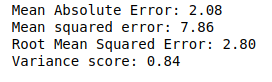
\includegraphics[width=0.5\textwidth]{./imagenes/MSE_Lineal.png}
        \end{center}

        % Ejercicio 7.b
        \item Comparando el MSE de este modelo con el del modelo anterior, 
        ¿cuál es menor? ¿a qué piensas que se debe?

        \textsc{Solución:}

    \end{enumerate}
\end{enumerate}
\end{document}
